\chapter{Prototype Pre-Alpha: Proof of Concept}

Pre-Alpha was theorized through the IPM model and intended as a "Proof of Concept" prototype. A Proof of Concept prototype is a realization of a certain method or idea in order to demonstrate its feasibility and functionality, or a demonstration in principle with the aim of verifying that some concept or theory has practical potential. \cite{poc}  Pre-Alpha was completed in the summer of 2016, see figure \ref{bachelorprototype2}. The sit-ski is made from 25x25x2.5mm AISI 316 SS profiles and ABS. The bottom mount is a combination of roller skies and mountain board trucks with off-road wheels as a steering system. The bottom mount is connected to the sit-ski with Rottefella bindings. This allows the mount to be attached to different sit-skis. Pre-Alpha's purpose was to prove whether or not the concept of sit-skiing with a steering system on bare-ground was possible. It described the functionality that a user might benefit from, with little attention to comfort and how the prototype would look. See "Bachelor Thesis; Steering system for cross-country sit-skis, 2016 NTNU" for the development process of Pre-Alpha.  

\vspace{0.5cm}
\begin{figure}[htb!]
    \centering
    {\setlength{\fboxsep}{0pt}\setlength{\fboxrule}{1pt}
    \fbox{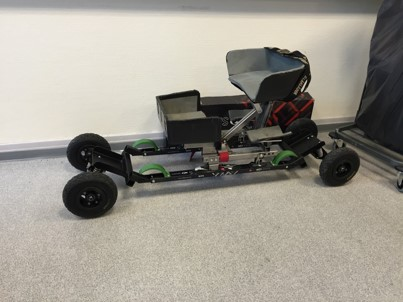
\includegraphics[height=0.35\textwidth]{figures/exero/bachelorprototype.jpg}}}
    \captionsetup{justification=centering}
    \caption{Pre-Alpha}
    \floatfoot{\textit{Source: Steering system for cross-country sit-skis} \cite{bachelorthesis}}
    \label{bachelorprototype2}
\end{figure}
\vspace{0.5cm}

\section{Testing and User Feedback}
Post-testing with disabled users confirmed the functionality of the Pre-Alpha concept. A Proof of Concept prototype is exhausted once the concept is proven successful. This allows the prototype to evolve to the next stage. Pre-Alpha was interchangeable between different sit-skis which allowed users to use their own sit-ski. The next prototype must be lighter and have better handling. This can be achieved through changing materials and strapping. 
\section{Discussion}
It is questionable whether or not the steering system and bottom mount should be sold as a complete package with one sit-ski or as a module to which multiple sit-skis can be mounted. Having a steering system that will fit with multiple cross-country sit-skis limits the expansion of the product because company sales will be limited by the number of cross-country sit-ski owners. 

%This deviates from what we concluded during the bachelor assignment which was that this product must not be limited for only cross-country users, but for all who have disabilities from the below the waist and has enough core muscle to move their torso.

It can also be argued that having a steering system that will fit with multiple cross-country sit-skis is a wise marketing choice for the early stages of the company. Exero wants to sell to a larger audience than that of cross-country sit-ski owners, though this is not certain. More research must be conducted to determine whether people without a sit-ski will have any interest in the product. 

%What we do know is that the users who already own a cross-country sit-ski and use it during the winter are very interested in this steering system we have developed. So maybe the best marketing choice in the beginning of the company is to focus on these users, and therefore make a steering system that will fit to multiple sit-skis. These are safe and certain customers that will buy and therefore build the company. Maybe once we are somewhat secured financially we can develop a product that is a whole package, or maybe we just do both?



%The overall  is that the Spike™ meets all functionality requirements, but more \textbf{adjustability} to satisfy every user. There must be more adjustments to individual parts. Also, feedback has been received on poor \textbf{visual design}, tighter \textbf{strapping} and more comfortable \textbf{seating}.